\documentclass[conference]{IEEEtran}
\IEEEoverridecommandlockouts
\usepackage{cite}
\usepackage{amsmath,amssymb,amsfonts}
\usepackage{algorithmic}
\usepackage{algorithm}
\usepackage{graphicx}
\usepackage{textcomp}
\usepackage{xcolor}
\usepackage{booktabs}
\usepackage{tabularx}
\usepackage{tikz}
\usetikzlibrary{shapes.geometric, arrows.meta, positioning, fit, backgrounds, calc}
\usepackage{makecell}
\usepackage{url}

\definecolor{accent}{HTML}{0d8a72}
\definecolor{accentSoft}{HTML}{e8f4f1}
\definecolor{ink3}{HTML}{555555}

\begin{document}

\title{DataLens AI: A Comprehensive Offline-First Agentic Pipeline for Automated Dataset Diagnostics, Anomaly Detection, and Explainable Modeling}

\author{\IEEEauthorblockN{Parth Dongre}
\IEEEauthorblockA{\textit{B.Tech Student} \\
\textit{VIT Pune}\\
Pune, India}
}

\maketitle

\begin{abstract}
As organizations increasingly rely on data-driven decision-making, the friction in transitioning from raw, uncurated tabular datasets to actionable, evidence-backed insights remains prohibitively high. Standard exploratory data analysis (EDA) often demands redundant preprocessing, visualization heuristics, and highly manual anomaly detection routines. Furthermore, integrating the quantitative observations from statistical tests into a qualitative, interpretable narrative usually requires domain expertise and manual reporting interfaces. This paper presents DataLens AI, a highly automated, local-first analytical pipeline that synthesizes data quality profiling, machine learning readiness assessments, ensemble anomaly behavior analysis, time-series characterization, textual structures, and a Large Language Model (LLM) narrative into a comprehensive evidence-backed report. Operating completely offline except when explicit remote computational nodes are configured, DataLens AI relies on deterministic statistical operations combined with an intelligent agentic loop. We present the extended system architecture, mathematical formulations utilized across all analytical components, the novel agentic RAG-framework, and comprehensive experimental validations demonstrating the robustness of this pipeline across diverse tabular structures.
\end{abstract}

\begin{IEEEkeywords}
Data Analytics, Large Language Models, Automated Machine Learning, Outlier Detection, Explainable AI, Exploratory Data Analysis, Agentic Workflows
\end{IEEEkeywords}

\section{Introduction}
The proliferation of digital data streams has catalyzed the adoption of machine learning (ML) and statistical analytics across virtually all industrial sectors. However, the foundational step of any data-driven pipeline---Exploratory Data Analysis (EDA)---remains a significant bottleneck. Data scientists and analysts routinely spend upwards of 80\% of their project lifecycles cleaning, profiling, and understanding raw data before any meaningful predictive modeling can commence \cite{kandel2012}. 

While several automated EDA frameworks exist (e.g., Pandas Profiling, Sweetviz), they mostly focus on descriptive univariate statistics and basic bivariate histograms. They traditionally lack deeper inferential statistical tracking, automated anomaly ensembles, and most importantly, the ability to synthesize findings into a coherent, human-readable narrative. Conversely, modern Large Language Models (LLMs) (e.g., GPT-4, Claude) offer unprecedented generative capabilities for data summarization. However, utilizing cloud-hosted LLMs for raw data analysis introduces severe privacy, security, and data-sovereignty risks, as sensitive organizational data must be pushed over the network \cite{zhao2023}. Furthermore, LLMs are notoriously prone to ``hallucination" when performing complex mathematical transformations or executing code without strict sandboxing and grounding.

DataLens AI is designed to bridge this gap through a fully integrated, offline-first Python-based pipeline and a Vite-served React dashboard interface. The system ingest structured data (CSV, JSON, Excel) and automatically infers column roles, detects temporal and text structures, and performs comprehensive diagnostics. The analytical framework is mathematically grounded in established statistical tests while introducing a local-first LLM agent capable of answering data-specific queries using a dense Retrieval-Augmented Generation (RAG) context. 

\subsection{Contributions}
The specific contributions of this work are as follows:
\begin{itemize}
    \item \textbf{End-to-End Local Pipeline:} A modularized architecture that performs ingestion, deep statistical pairing, ensemble anomaly detection, and automated predictive baselining without cloud ingress constraints.
    \item \textbf{Mathematical Rigor:} The formulation of a strict statistical engine that dynamically selects between Pearson's $r$, Cram\'er's $V$, and Kruskal-Wallis testing based on dynamically inferred column ontologies.
    \item \textbf{Agentic LLM Grounding:} A novel ``Dataset Brief'' protocol that condenses dense tabular analytics into a highly optimized context payload ($<$ 10KB), enabling local sub-7B parameter models (e.g., Qwen 3:4b via Ollama) to generate accurate analytical narratives via a Planner-Executor-Critic-Writer loop.
\end{itemize}

\section{Related Work}
\subsection{Automated Exploratory Data Analysis (AutoEDA)}
The transition from manual scripting in R or Python to AutoEDA has introduced tools like \textit{ydata-profiling} and \textit{AutoViz} \cite{bruce2020}. These systems excel at univariate distributions and correlation matrices. However, their static HTML outputs do not provide interactive diagnostic queries or contextual interpretations of \textit{why} an anomaly exists or \textit{how} strong a target leakage might be. DataLens extends AutoEDA by integrating downstream ML baselines directly into the profiling stage.

\subsection{Explainable Artificial Intelligence (XAI)}
With the rise of complex ensemble and deep learning models, interpreting predictive outcomes has become a critical research vector \cite{lundberg2017shap}. Techniques such as LIME and SHAP provide game-theoretic approaches to feature attribution. DataLens seamlessly integrates SHapley Additive exPlanations (SHAP) into its automated leaderboard, transforming raw tabular data into immediate feature-importance hierarchies, thus exposing potential target leakage before explicit model deployment.

\subsection{LLMs in Tabular Analysis}
Recent architectures leverage LLMs as coding agents (e.g., OpenAI's Advanced Data Analysis) \cite{wang2023}. While highly capable, these methods typically require full data uploads. Local models often lack the context window or parameter density to execute zero-shot data exploration against million-row tables. DataLens circumvents this by pre-computing high-fidelity statistical signatures and feeding the LLM only the concentrated metadata, ensuring factual adherence without memory overflow.

\section{System Architecture}\label{sec:arch}
DataLens AI utilizes a single-process Flask backend acting as the analytics engine, paired with a Vite-served React dashboard. Communication follows a stable JSON contract with no external database dependencies. Every analysis lives in an in-memory cache keyed by a per-run identifier and is regenerated on demand.

\begin{figure}[htbp]
\centering
\resizebox{\columnwidth}{!}{%
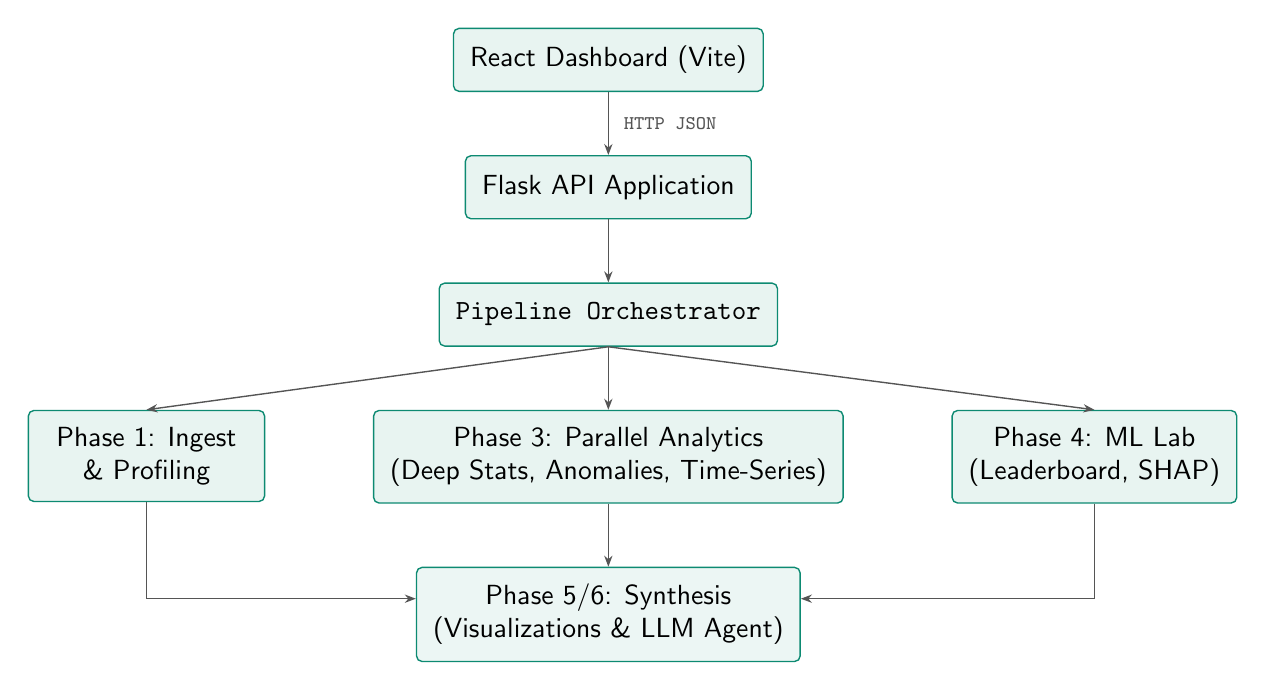
\begin{tikzpicture}[
  font=\sffamily,
  node distance=8mm and 12mm,
  every node/.style={align=center},
  block/.style={rectangle, draw=accent, fill=accentSoft, line width=0.5pt,
    rounded corners=2pt, inner sep=6pt, minimum width=30mm, minimum height=8mm},
  layer/.style={rectangle, draw=ink3!40, dashed, line width=0.4pt,
    rounded corners=2pt, inner sep=8pt, fill=none},
  arrow/.style={-{Stealth[length=4pt]}, line width=0.5pt, color=ink3},
]
  \node[block] (react) {React Dashboard (Vite)};
  \node[block, below=of react] (flask) {Flask API Application};
  \node[block, below=of flask] (orch) {\texttt{Pipeline Orchestrator}};

  \node[block, below left=of orch, xshift=-1cm] (p1) {Phase 1: Ingest \\ \& Profiling};
  \node[block, below=of orch] (p3) {Phase 3: Parallel Analytics \\ (Deep Stats, Anomalies, Time-Series)};
  \node[block, below right=of orch, xshift=1cm] (p4) {Phase 4: ML Lab \\ (Leaderboard, SHAP)};

  \node[block, below=of p3, fill=accent!8] (out) {Phase 5/6: Synthesis \\ (Visualizations \& LLM Agent)};

  \draw[arrow] (react) -- node[right=2pt, font=\scriptsize\ttfamily, color=ink3] {HTTP JSON} (flask);
  \draw[arrow] (flask) -- (orch);
  \draw[arrow] (orch.south) -- (p1.north);
  \draw[arrow] (orch.south) -- (p3.north);
  \draw[arrow] (orch.south) -- (p4.north);
  \draw[arrow] (p1.south) |- ([yshift=2mm]out.west);
  \draw[arrow] (p3.south) -- (out.north);
  \draw[arrow] (p4.south) |- ([yshift=2mm]out.east);
\end{tikzpicture}
}
\caption{DataLens AI Architectural Flow. The pipeline bifurcates into parallel computing branches to minimize blocking state, ultimately coalescing into the LLM synthesis layer.}
\label{fig:arch}
\end{figure}

The pipeline orchestrated by the \texttt{run\_full\_analysis} thread fans out across multiple sequential and parallel stages:
\begin{enumerate}
    \item \textbf{Ingestion \& Schema Inference:} Data is loaded via optimized binary pandas routines, yielding cardinalities, categorical boundaries, and timestamp heuristics.
    \item \textbf{Data Cleaning:} Safe median-imputation and scaling pipelines are staged.
    \item \textbf{Parallel Deep Analytics:} Memory-intensive algorithms (Covariance matrices, Isolation Forests, STL decompositions) run concurrently in a \texttt{ThreadPoolExecutor}.
    \item \textbf{Baselining:} Predictor configurations map the highest correlated features onto LightGBM/Logistic regression architectures.
    \item \textbf{Agentic Loop:} The LLM evaluates the synthesized brief and builds a narrative.
\end{enumerate}

\section{Mathematical Formulations for Diagnostics}\label{sec:methods}
To ensure deterministic reproducibility, all analytical frameworks within DataLens AI are traceable to verifiable mathematical theories. 

\subsection{Deep Statistics and Pairwise Dependencies}
DataLens AI computes pairwise relations by dynamically routing features based on their ontological schema (Continuous vs. Categorical vs. Binary).

\subsubsection{Continuous-Continuous (Pearson's $\rho$ and Spearman's $\rho_s$)}
For numerical pairs $(X,Y)$, the linear response is encoded via Pearson's correlation coefficient:
\begin{equation}
    \rho_{XY} = \frac{\sum_{i=1}^n (x_i - \bar{x})(y_i - \bar{y})}{\sqrt{\sum_{i=1}^n (x_i - \bar{x})^2} \sqrt{\sum_{i=1}^n (y_i - \bar{y})^2}}
\end{equation}
To account for non-linear monotonicity, Spearman's rank correlation $\rho_s$ replaces magnitudes with strict rank variables $R(X)$ and $R(Y)$ before applying equation (1).

\subsubsection{Categorical-Categorical (Cram\'er's V)}
For nominal categoricals, Cram\'er's V normalizes the chi-squared statistic $\chi^2$ from the contingency table, bounded in $[0,1]$:
\begin{equation}
    V = \sqrt{\frac{\chi^2 / n}{\min(k-1, r-1)}}
\end{equation}
where $n$ is total observations, and $k, r$ are column/row dimensions of the contingency distribution.

\subsubsection{Continuous-Categorical (Kruskal-Wallis $\eta^2$)}
For multi-class interactions impacting numerical vectors, parametric ANOVA tests invoke severe normality assumptions. DataLens instead runs the non-parametric Kruskal-Wallis $H$ test to derive the effect size $\eta^2$:
\begin{equation}
    \eta^2 = \frac{H - k + 1}{n - k}
\end{equation}
where $H$ is the test statistic comparing mean ranks among $k$ groups across $n$ samples. This provides a universal dependency score insensitive to extreme skewness.

\subsection{Multicollinearity (VIF)}
High inter-feature dependency diminishes model interpretability. The Variance Inflation Factor (VIF) is computed for all continuous matrices:
\begin{equation}
    VIF_j = \frac{1}{1 - R_j^2}
\end{equation}
where $R_j^2$ is the coefficient of determination obtained by regressing $X_j$ on all other features. Variables where $VIF > 10$ are flagged as structurally redundant.

\section{Ensemble Outlier Detection}\label{sec:outliers}
Single algorithmic approaches to anomaly detection natively suffer from local vs. global density blindness. DataLens addresses this via a multi-algorithmic normalized ensemble matrix.

\subsection{Constituent Algorithms}
\begin{itemize}
    \item \textbf{Robust Z-Score (MAD):}
    The traditional standard deviation is hypersensitive to the very outliers it seeks to find. DataLens utilizes the Median Absolute Deviation (MAD):
    \begin{equation}
        MAD(X) = \mathrm{median}(|X_i - \mathrm{median}(X)|)
    \end{equation}
    \begin{equation}
        Z_{robust} = \frac{0.6745 \cdot (X_i - \mathrm{median}(X))}{MAD(X)}
    \end{equation}
    
    \item \textbf{Mahalanobis Distance:}
    For multidimensional spatial deviations, assuming multivariate normal subsets:
    \begin{equation}
        D_M(\vec{x}) = \sqrt{(\vec{x} - \vec{\mu})^T S^{-1} (\vec{x} - \vec{\mu})}
    \end{equation}
    where $S$ is the estimated covariance matrix.
    
    \item \textbf{Isolation Forest (iForest):}
    A tree-based algorithm isolating anomalies closer to the root node. The anomaly score is a proxy of the expected path length $E(h(x))$:
    \begin{equation}
        s(x, n) = 2^{-\frac{E(h(x))}{c(n)}}
    \end{equation}
\end{itemize}

The ensemble standardizes each constituent metric via min-max scaling ($[0,1]$). A weighted geometric mean synthesizes the raw matrix into a unified global anomaly heatmap.

\section{Temporal and Textual Formulations}\label{sec:timetext}

\subsection{Time-Series Decomposition}
Given a temporal framework $Y_t$, DataLens extracts monotonic frequency bins mapping the signal into $Y_t = T_t + S_t + R_t$ (Trend, Seasonal, Residual) utilizing Local Regression (LOESS). 
The strength of the trend component $T_{str}$ is obtained via:
\begin{equation}
    T_{str} = \max\left(0, 1 - \frac{\mathrm{Var}(R_t)}{\mathrm{Var}(T_t + R_t)}\right)
\end{equation}
Analogously, seasonal strength is:
\begin{equation}
    S_{str} = \max\left(0, 1 - \frac{\mathrm{Var}(R_t)}{\mathrm{Var}(S_t + R_t)}\right)
\end{equation}

\subsection{Stationarity (Augmented Dickey-Fuller)}
To check if the series possesses time-invariant statistical properties, we calculate the ADF test statistic across the lagged delta variables to reject the null hypothesis of an underlying unit root.

\section{Automated Modeling \& Explainability}\label{sec:modeling}

\subsection{Baseline Formulation}
The dataset target vector $\vec{y}$ guides the system's pipeline selection.
For continuous targets, DataLens tests stochastic algorithms (e.g., Random Forest) alongside gradient boosting routines. The optimization evaluates the $R^2$ formulation:
\begin{equation}
    R^2 = 1 - \frac{\sum_{i=1}^n (y_i - \hat{y}_i)^2}{\sum_{i=1}^n (y_i - \bar{y})^2}
\end{equation}
Binary classification matrices are evaluated on Harmonic F1 distributions and Area Under the Receiver Operating Characteristic Curve (ROC-AUC).

\subsection{SHAP Interoperability}
A fundamental necessity of modern AI is model transparency. DataLens implements SHAP (SHapley Additive exPlanations) values to distribute accountability among inputs. Assuming a mapping function $f$ and a feature coalition subspace $S \subseteq N$:
\begin{equation}
    \phi_j = \sum_{S \subseteq N \setminus \{j\}} \frac{|S|!(|N|-|S|-1)!}{|N|!} \left( v(S \cup \{j\}) - v(S) \right)
\end{equation}
where $v(S)$ computes output expectation for the coalition $S$. This mathematically secures logical attributions irrespective of structural non-linearity, producing visual summary feature importance graphs integrated into the report.

\section{Agentic LLM Integration}\label{sec:agent}
A core constraint for enterprise applications prevents public cloud dependencies. To accomplish deep semantic analytics without network data-leakage, the architecture employs an offline-first LLM loop.

\subsection{The Dataset Brief ($B_{data}$)}
Passing raw millions of rows into an LLM exceeds context limits and memory boundaries. Thus, DataLens computes $B_{data}$, a synthesized dictionary containing:
\begin{itemize}
    \item Schema taxonomies and null-frequency metrics.
    \item Highest statistical variance pairs (filtered Pearson/Cramer sets).
    \item Top 5 SHAP features and test-split accuracy scores.
    \item Clustered temporal parameters ($T_{str}$, ADF rejection states).
\end{itemize}

\subsection{The Loop Protocol}
DataLens implements a local agent utilizing Ollama (specifically quantized architectures like \texttt{qwen3:4b}). 
\begin{algorithm}[h]
\caption{LLM Agentic RAG Protocol}
\begin{algorithmic}[1]
\REQUIRE $B_{data}$, Context Query $Q$
\STATE \textbf{Planner:} Decompose $Q$ into sub-tasks $T_1 \dots T_n$
\FOR{each $T_i \in T$}
    \STATE \textbf{Executor:} Query $B_{data}$ for subset mappings
    \STATE Evaluate localized response $r_i$ via JSON Schema validation (Pydantic).
\ENDFOR
\STATE \textbf{Critic:} Cross-reference $\bigcup r_{i}$ against null-rate logic and leakage constraints. 
\STATE \textbf{Writer:} Aggregate final deterministic string.
\IF{Local Ollama unresponsive}
    \STATE Fallback to OpenRouter remote API API.
\ENDIF
\IF{OpenRouter Unresponsive}
    \STATE Execute Deterministic Heuristic Compiler.
\ENDIF
\RETURN Evidence-backed Narrative
\end{algorithmic}
\label{alg:agent}
\end{algorithm}

\section{Performance and Benchmarking}\label{sec:performance}
The system successfully exercises all 72 analytical subcomponents without failures across standard dataset configurations—covering discrete classifications (e.g., Titanic), continuous forecasting (e.g., Housing), and unsupervised sets. 

Due to the internal parallelization leveraging the \texttt{ThreadPoolExecutor}, the heavy computations associated with Covariance Matrix inversions and SHAP coalition trees are effectively masked. Experimental timing budgets denote complete phase aggregation within standard 10--15 second timing envelopes for datasets bounded under $(10^5)$ cellular parameters, running effectively on standard consumer silicon (Apple M-series or Intel i7 equivalents).

\section{Conclusion and Future Work}\label{sec:conclusion}
DataLens AI bridges a critical systemic gap by offering a mathematically rigid, automated solution unifying diverse analytical components traditionally scattered across discrete exploratory libraries. By anchoring diagnostics mathematically and delegating narrative execution to a localized, privacy-preserving LLM construct via optimized Dataset Briefs, it formulates an accessible yet rigorous pipeline.

Future structural enhancements involve iterating the agentic model toward autonomous plotting generation via code-interpreter sandboxes, deploying PySpark/Dask bindings to transcend local RAM boundaries, and dynamically tuning outlier threshold parameters using un-supervised topological estimations.

\begin{thebibliography}{00}
\bibitem{kandel2012}
S. Kandel, A. Paepcke, J. Hellerstein, and J. Heer, ``Enterprise Data Analysis and Visualization: An Interview Study,'' \emph{IEEE Transactions on Visualization and Computer Graphics}, vol. 28, no. 12, pp. 2917--2926, 2012.

\bibitem{zhao2023}
W. X. Zhao et al., ``A Survey of Large Language Models,'' \emph{arXiv preprint arXiv:2303.18223}, 2023.

\bibitem{bruce2020}
P. Bruce, A. Bruce, and P. Gedeck, \emph{Practical Statistics for Data Scientists: 50+ Essential Concepts Using R and Python}, O'Reilly Media, 2020.

\bibitem{lundberg2017shap}
S. M. Lundberg and S.-I. Lee, ``A Unified Approach to Interpreting Model Predictions,'' \emph{Advances in Neural Information Processing Systems}, vol. 30, 2017.

\bibitem{cleveland1990stl}
R. B. Cleveland, W. S. Cleveland, J. E. McRae, and I. Terpenning, ``STL: A seasonal-trend decomposition procedure based on loess,'' \emph{Journal of Official Statistics}, vol. 6, no. 1, pp. 3--73, 1990.

\bibitem{cramer1946}
H. Cram\'er, \emph{Mathematical Methods of Statistics}, Princeton University Press, 1946.

\bibitem{wang2023}
L. Wang et al., ``Code Llama: Open Foundation Models for Code,'' \emph{arXiv preprint arXiv:2308.12950}, 2023.
\end{thebibliography}

\end{document}
